\documentclass[a4paper]{article}
\usepackage{amsmath}
\usepackage{amssymb}
\usepackage{pgf}
\usepackage{tikz}
\usepackage{tikz-3dplot}
\usetikzlibrary{decorations.markings}
\tikzset{middlearrow/.style={
        decoration={markings,
            mark= at position 0.5 with {\arrow{#1}} ,
        },
        postaction={decorate}
    }
}
\usetikzlibrary{calc,cd}

\begin{document}

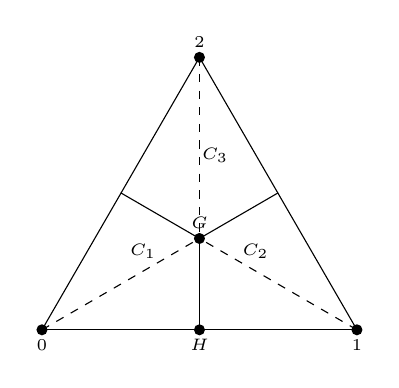
\begin{tikzpicture}[scale=2,font=\fontsize{6}{6}\selectfont]
          \fill[color=black] (0,0) circle(1pt) node[below] {$0$};
          \fill[color=black] (2,0) circle(1pt) node[below] {$1$};
          \fill[color=black] (1,1.73) circle(1pt) node[above] {$2$};
           \fill[color=black] (1,0.58) circle(1pt) node[above] {$G$};
           \fill[color=black] (1,0) circle(1pt) node[below] {$H$};
           \draw (0,0) -- (2,0);
           \draw (0,0) -- (1,1.73);
           \draw (2,0) -- (1,1.73);
           \draw (0.5,0.87) -- (1,0.58);
           \draw (1.5,0.87) -- (1,0.58);
           \draw (1,0) -- (1,0.58);
           \draw (0.5,0.5) node[right] {$C_1$};
           \draw (1.5,0.5) node[left] {$C_2$};
           \draw (1.1,1) node[above] {$C_3$};
           \draw [dashed] (0,0) -- (1,0.58);
           \draw [dashed] (1,1.73) -- (1,0.58);
           \draw [dashed] (2,0) -- (1,0.58);
         \end{tikzpicture}

\end{document}